\documentclass[../main.tex]{subfiles}

\begin{document}
	Il sistema $ S $ \'e costituito da $ N $ sottosistemi $ S^{(i)} $ con $ i = 1...N $, ognuno con il suo vettore $ \vec x^{(i)} $.
	\[
		\begin{aligned}
			&\text{vettore degli ingressi esogeni}
			\\
			&\vec u =
			\begin{bmatrix}
				u_1\\
				\vdots\\
				u_{n_u}
			\end{bmatrix}
		\end{aligned}
		\qquad\qquad
		\begin{aligned}
			&\text{vettore degli uscite}
			\\
			&\vec y =
			\begin{bmatrix}
				y_1\\
				\vdots\\
				y_{n_y}
			\end{bmatrix}
		\end{aligned}
	\]
	\[
		\begin{aligned}
			&\text{vettore degli ingressi di $ S^{(i)} $}
			\\
			&\vec u =
			\begin{bmatrix}
				u_1\\
				\vdots\\
				u_{n_u}
			\end{bmatrix}
		\end{aligned}
		\qquad\qquad
		\begin{aligned}
			&\text{vettore degli uscite di $ S^{(i)} $}
			\\
			&\vec y =
			\begin{bmatrix}
				y_1\\
				\vdots\\
				y_{n_y}
			\end{bmatrix}
		\end{aligned}
	\]
	
	\section{Studio delle propriet\'a strutturali}
		\begin{enumerate}
			\item 
				Mettere in equazione di stato ogni singolo sistema $ S^{(i)} $ con realizzazione minima
				\[
					S^{(i)}:
					\begin{cases}
						\dot{\vec x}^{(i)} = A^{(i)} \vec x^{(i)} + B^{(i)} \vec u^{(i)}\\
						\dot{\vec y}^{(i)} = C^{(i)} \vec x^{(i)} + D^{(i)} \vec u^{(i)}
					\end{cases}
				\]
			\item 
				Scrivo le equazioni di interconnessione, cio\'e esprimo $ \vec u^{(i)} $ e $ \vec y $ come funzione (combinazione lineare) di tutte le uscite $ \vec y^{(i)} $ e di tutti gli ingressi esogeni $ \vec u $.
			\item 
				Per sostituzioni successive, elimino le dipendenze da $ \vec u^{(i)} $ e da $ \vec y^{(i)} $. Otteniamo un sistema lineare:
				\[
					\begin{cases}
						\dot{\vec x} = A \vec x + B \vec u\\
						\vec y = C \vec x + D \vec u
					\end{cases}
				\]
				NB: non devono essere presenti loop algebrici, altrimenti questo passaggio non ha fine.
			\item 
				Studio delle propriet\'a strutturali (Controllabilit\'a, Osservabilit\'a, Stabilit\'a) del sistema di equazioni di stato cos\'i ottenuto
		\end{enumerate}
	
		\paragraph{Esempio}
			\[
				\begin{aligned}
					T^{(1)}(s) = \dfrac{1}{s+1}
					&\quad\Rightarrow\quad
					\varphi_{CO}^{(1)}(s) = s+1
					\\
					T^{(2)}(s) = \dfrac{s+1}{s}
					&\quad\Rightarrow\quad
					\varphi_{CO}^{(2)}(s) = s
				\end{aligned}
			\]
			Si tratta di un sistema di ordine 2. Eseguiamo tutti i passaggi:
			\begin{enumerate}
				\item 
					\[
						S^{(1)}:
						\begin{cases}
							\dot x^{(1)} = -x^{(1)} + u^{(1)}\\
							y^{(1)} = x^{(1)}
						\end{cases}
						\qquad
						S^{(2)}:
						\begin{cases}
							\dot x^{(2)} = u^{(2)}\\
							y^{(2)} = x^{(2)} + u^{(2)}
						\end{cases}
					\]
				\item 
					\[
						u^{(1)} = u \qquad u^{(2)} = y^{(1)} \qquad y = y^{(2)}
					\]
				\item 
					\[
						\begin{aligned}
							\dot x^{(1)} &= -x^{(1)} + u\\
							y^{(1)} &= x^{(1)}\\
							\dot x^{(2)} &= y^{(1)} = x^{(1)}\\
							y^{(2)} &= x^{(2)} + y^{(1)} = x^{(2)} + x^{(1)}\\
							y &= y^{(2)} = x^{(2)} + u^{(2)} = x^{(2)} + y^{(1)} = x^{(2)} + x^{(1)}
						\end{aligned}
					\]
					\[
						\Rightarrow\quad S:
						\begin{cases}
							\dot{\vec x} =
							\begin{bmatrix}
								-1 & 0\\
								1 & 0
							\end{bmatrix} \vec x +
							\begin{bmatrix}
								1\\
								0
							\end{bmatrix} u
							\\
							y =
							\begin{bmatrix}
								1 & 1
							\end{bmatrix} \vec x
						\end{cases}
					\]
				\item 
					\[
						\varphi(s) = det(sI-A) = det
						\begin{bmatrix}
							s+1 & 0\\
							-1 & s
						\end{bmatrix} = s(s+1)
						\qquad
						m(s) \equiv \varphi(s)\ \text{perch\'e}\ m(s) \subseteq\cdot \varphi(s)
					\]
					Il sistema \'e semplicemente stabile perch\'e c'\'e un autovalore a $ \Re = 0 $ e uno a $ \Re < 0 $
					\[
						P =
						\begin{bmatrix}
							1 & | & -1\\
							0 & | & 1
						\end{bmatrix}
						\quad\Rightarrow\quad
						rank(P) = 2
					\]
					Il sistema \'e completamente controllabile.
					\[
						Q =
						\begin{bmatrix}
							1 & 1\\
							\cline{1-2}
							0 & 0
						\end{bmatrix}
						\quad\Rightarrow\quad
						rank(Q) = 1
					\]
					Il sistema non \'e completamente osservabile.
					\[
						(sI-A)^{-1} =
						\begin{bmatrix}
							\dfrac{1}{s+1} & 0\\[.5cm]
							\dfrac{1}{s(s+1)} & \dfrac{1}{s}
						\end{bmatrix}
					\]
					\[
						(sI-A)^{-1}B =
						\begin{bmatrix}
							\dfrac{1}{s+1}\\[.5cm]
							\dfrac{1}{s(s+1)}
						\end{bmatrix}
						\quad\Rightarrow\quad
						\varphi_C(s) = s(s+1)
					\]
					\[
						C(sI-A)^{-1} = 
						\begin{bmatrix}
							\dfrac{1}{s+1}+\dfrac{1}{s(s+1)} & \dfrac{1}{s}
						\end{bmatrix} =
						\begin{bmatrix}
							\dfrac{1}{s} & \dfrac{1}{s}
						\end{bmatrix}
						\quad\Rightarrow\quad
						\varphi_O(s) = s
					\]
			\end{enumerate}
		
			\begin{Exercise}[title={Studiare propriet\'a di sistemi interconnessi}, difficulty=3]
				Sono dati i sistemi:
				\[
					S^{(1)}:
					\begin{cases}
						\dot{\vec x}^{(1)} =
						\begin{bmatrix}
							0 & 1\\
							-1 & 2
						\end{bmatrix}
						\vec x^{(1)} +
						\begin{bmatrix}
							0\\
							1
						\end{bmatrix} u^{(1)}
						\\[.5cm]
						y^{(1)} =
						\begin{bmatrix}
							1 & 1\\
							0 & 1
						\end{bmatrix} \vec x^{(1)}
					\end{cases}
				\]
				\[
					S^{(2)}: T(s)^{(2)}=\dfrac{1}{s+1}
				\]
				
				\begin{center}
					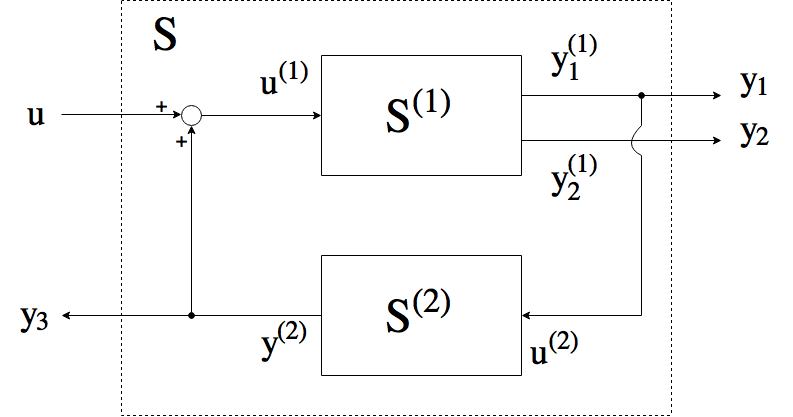
\includegraphics[width=.7\textwidth]{sistemi_interconnessi/esercizio_sistemi_interconnessi}	
				\end{center}
				
				Sono due sistemi strettamente propri quindi non ci sono loop algebrici. Metto in equazione di stato il 2° sistema:
				\[
					S^{(2)}:
					\begin{cases}
						\dot x^{(2)} = -x^{(2)} + u^{(2)}\\
						y^{(2)} = x^{(2)}
					\end{cases}
				\]
				\begin{enumerate}
					\item 
						\begin{align*}
							\dot x^{(1)}_1 &= x^{(1)}_2\\
							\dot x^{(1)}_2 &= -x^{(1)}_1 + 2x^{(1)}_2 + u^{(1)}\\
							y^{(1)}_1 &= x^{(1)}_1 + x^{(1)}_2\\
							y^{(1)}_2 &= x^{(1)}_2
						\end{align*}
					\item 
						\begin{align*}
							u^{(1)} &= y^{(2)} + u\\
							u^{(2)} &= y^{(1)}_1\\
							y_1 &= y^{(1)}_1\\
							y_2 &= y^{(1)}_2\\
							y_3 &= y^{(2)}
						\end{align*}
					\item 
						\begin{align*}
							\dot x^{(1)}_2 &= -x^{(1)}_1 + 2x^{(1)}_2 + y^{(2)} + u = -x^{(1)}_1 + 2x^{(1)}_2 + x^{(2)} + u\\
							\dot x^{(2)} &= -x^{(2)} + y^{(1)}_1 = -x^{(2)} + x^{(1)}_1 + x^{(1)}_2\\
							y_1 &= x^{(1)}_1 + x^{(1)}_2\\
							y_2 &= x^{(1)}_2\\
							y_3 &= x^{(2)}
						\end{align*}
						\[
							\begin{aligned}
								\dot{\vec x} &= 
								\begin{bmatrix}
									0 & 1 & 0\\
									-1 & 2 & 1\\
									1 & 1 & -1
								\end{bmatrix} \vec x+
								\begin{bmatrix}
									0\\
									1\\
									0
								\end{bmatrix} u
								\\
								\vec y &= 
								\begin{bmatrix}
									1 & 1 & 0\\
									0 & 1 & 0\\
									0 & 0 & 1
								\end{bmatrix} \vec x +
								\begin{bmatrix}
									0\\
									0\\
									0
								\end{bmatrix} u
							\end{aligned}
						\]
					\item 
						\begin{itemize}
							\item Controllabilit\'a:
								\[
									P=
									\begin{bmatrix}
										0 &|& 1 &|& 2\\
										1 &|& 2 &|& 4\\
										0 &|& 1 &|& 2
									\end{bmatrix}
									\quad\Rightarrow\quad
									rank(P) =2
								\]
							\item Osservabilit\'a:
								\[
									Q=
									\begin{bmatrix}
										1 & 1 & 0\\
										0 & 1 & 0\\
										0 & 0 & 1\\
										\cline{1-3}\\
										&\dots&
									\end{bmatrix}
								\]
								Poich\'e gi\'a $ rank(C) = 3 $, il sistema \'e completamente osservabile.
								
								Calcoliamo completamente $ Q $ per studiare l'osservabilit\'a da ogni singola uscita:
								\[
									Q=
									\begin{bmatrix}
										1 & 1 & 0\\
										0 & 1 & 0\\
										0 & 0 & 1\\
										\cline{1-3}\\
										-1 & 3 & 1\\
										-1 & 2 & 1\\
										1 & 1 & -1\\
										\cline{1-3}\\
										-2 & 6 & 2\\
										-1 & 4 & 1\\
										-2 & 2 & 2
									\end{bmatrix}
								\]
								Le prime righe di ogni sottomatrice non sono linearmente indipendenti, quindi il sistema non \'e completamente osservabile da $ y_1 $.\\
								Le seconde righe di ogni sottomatrice non sono linearmente indipendenti, quindi il sistema non \'e completamente osservabile da $ y_2 $.\\
								Le terze righe di ogni sottomatrice sono linearmente indipendenti(bisogna calcolare tutti i minori), quindi il sistema non \'e completamente osservabile da $ y_3 $.\\
							\item Stabilit\'a:
								\[
									\varphi(s) = det
									\begin{bmatrix}
										s & -1 & 0\\
										1 & s-2 & -1\\
										-1 & -1 & s+1
									\end{bmatrix} =
									(-s-1)+(s+1)(s^2-2s+1) = (s+1)(s^2-2s+1-1) =(s+1)s(s-2)
								\]
								poich\'e $ m(s) \subseteq\cdot \varphi(s) $, allora $ m(s) \equiv \varphi(s) $. Il sistema \'e instabile.
							\item Stabilit\'a BIBO:\\
								se nella matrice di trasferimento scompaiono gli autovalori $ 0 $ e $ +2 $, sarebbe stabile BIBO, cio\'e se $ \varphi_{CO}(s) = \dfrac{1}{s+1} $ o $ \varphi_{CO}(s) = 1 $. Ma abbiamo trovato che $ \pDeg{\varphi_C(s)} = 2 $ e $ \pDeg{\varphi_{O}(s)} = 3 $, quindi $ \pDeg{\varphi_{CO}(s)} = 2 $ (\'e l'intersezione dei gradi $ \varphi_C(s) $ e $ \varphi_O(s) $), cio\'e conterr\'a almeno uno di quei due autovalori ($ 0 $ o $ +2 $). Il sistema \'e instabile BIBO.
						\end{itemize}
				\end{enumerate}
			\end{Exercise}
	
		Molte delle propriet\'a strutturali possono essere desunte sfruttando relazioni note tra i polinomi.
		\paragraph{Esempio}
			\[
				T(s) = \dfrac{1}{s^2}
			\]
			\begin{itemize}
				\item Stabilit\'a BIBO:\\
					non \'e stabile perch\'e c'\'e una radice a $ \Re = 0 $
				\item Stabilit\'a:\\
					\[
						\varphi_{CO}(s) = s^2 \equiv m_{CO}(s)
					\]
					\begin{itemize}
						\item 
							$ \varphi_{CO}(s) \subseteq \varphi(s) $ ($ s^2 \subseteq \varphi(s) $) allora $ \varphi(s) $ avr\'a una radice a $ \Re = 0 $. Il sistema non pu\'o essere asintoticamente stabile.
						\item 
							$ m_{CO}(s) \subseteq m(s) $ ($ s^2 \subseteq m(s) $) allora $ m(s) $ ha una radice a $ \Re = 0 $ con molteplicit\'a 2. Il sistema \'e instabile.
					\end{itemize}
			\end{itemize}
		
	\section{Sistemi serie/parallelo}
		Il polinomio caratteristico di polinomi connessi unicamente serie e/o parallelo \'e dato dal prodotto dei singoli polinomi caratteristici.
		\paragraph{Dimostrazione serie}
			\[
				S^{(1)}:
				\begin{cases}
					\dot x^{(1)} = A^{(1)} x^{(1)} + B^{(1)} u^{(1)}\\
					y^{(1)} = C^{(1)} x^{(1)} + D^{(1)} u^{(1)}
				\end{cases}
				\qquad
				S^{(2)}:
				\begin{cases}
					\dot x^{(2)} = A^{(2)} x^{(2)} + B^{(2)} u^{(2)}\\
					y^{(2)} = C^{(2)} x^{(2)} + D^{(2)} u^{(2)}
				\end{cases}
			\]
			\begin{figure}[h!]
				\centering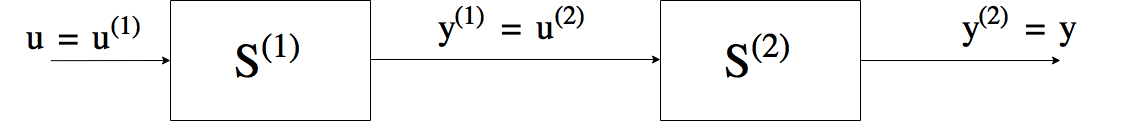
\includegraphics[width=.7\textwidth]{sistemi_interconnessi/dimostrazione_serie}
			\end{figure}
		
			Le equazioni di interconnessione sono:
			\[
				u^{(2)} = y^{(1)} \qquad u^{(1)} = u \qquad y = y^{(2)}
			\]
			quindi sostituendo nel secondo sistema otteniamo:
			\[
				\begin{aligned}
					\dot x^{(2)} &= A^{(2)} x^{(2)} + B^{(2)} \left[ C^{(1)} x^{(1)} + D^{(1)} u \right] = A^{(2)} x^{(2)} + B^{(2)} c^{(1)} x^{(1)} + B^{(2)} D^{(1)} u
					\\
					y^{(2)} &= C^{(2)} x^{(2)} + D^{(2)} C^{(1)} x^{(1)} + D^{(2)} D^{(1)} u
				\end{aligned}
			\]
			\[
				\begin{cases}
						\dot{\vec x} =
						\begin{bmatrix}
							A^{(1)} & 0\\
							B^{(2)} C^{(1)} & A^{(2)}
						\end{bmatrix} \vec x +
						\begin{bmatrix}
							B^{(1)}\\
							B^{(2)} D^{(1)}
						\end{bmatrix} \vec u
						\\
						\vec y =
						\begin{bmatrix}
							D^{(2)} C^{(2)} & C^{(2)}
						\end{bmatrix} \vec x + 
						D^{(2)} D^{(1)} \vec u
				\end{cases}
			\]
			$ A_{serie} $ \'e una matrice triangolare a blocchi quindi:
			\[
				\varphi_{serie}(s) = det(sI-A_{serie}) = det(sI-A^{(1)}) \cdot det(sI-A^{(2)}) = \varphi^{(1)}(s) \cdot \varphi^{(2)}(s)
			\]
		\paragraph{Parallelo}
			\[
				\dot{\vec x} = 
				\begin{bmatrix}
					A^{(1)} & 0\\
					0 & A^{(2)}
				\end{bmatrix} \vec x +
				\begin{bmatrix}
					B^{(1)}\\
					B^{(2)}
				\end{bmatrix} u
				\\
				y = 
				\begin{bmatrix}
					C^{(1)} & C^{(2)}
				\end{bmatrix} \vec x +
				\left( D^{(1)} + D^{(2)} \right) u
			\]
			\begin{figure}[h!]
				\centering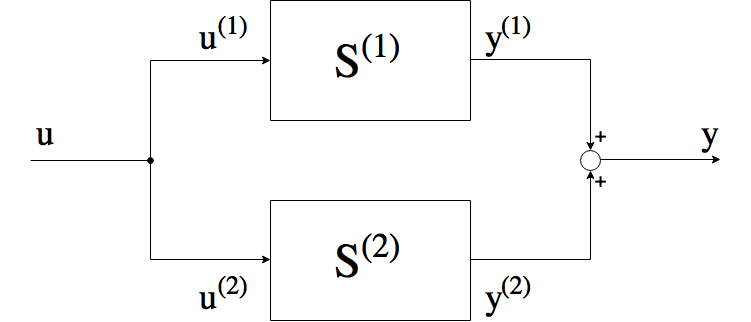
\includegraphics[width=.7\textwidth]{sistemi_interconnessi/dimostrazione_parallelo}
			\end{figure}
		
			$ A_{parallelo} $ \'e una matrice diagonale:
			\[
				det(sI-A_{parallelo}) = det(sI-A^{(1)}) \cdot det(sI-A^{(2)}) = \varphi_{parallelo}(s) = \varphi^{(1)}(s) \cdot \varphi^{(2)}(s)
			\]
	\subsection{Corollario}
		Condizione necessaria e sufficiente per asintotica stabilit\'a di un sistema serie e/o parallelo \'e l'asintotica stabilit\'a dei singoli sistemi. Non vale per la semplice stabilit\'a.
		
	\subsection{Propriet\'a di controllabilit\'a e osservabilit\'a}
		Condizione necessaria per la controllabilit\'a (osservabilit\'a) di un sistema interconnesso \'e che tutti i suoi possibili sottosistemi siano controllabili (osservabili).
		
		Si consideri un sistema interconnesso $ S $ formato da $ N $ sottosistemi, ognuno dei quali \'e completamente controllabile e osservabile.
		
		\begin{figure}[h!]
			\centering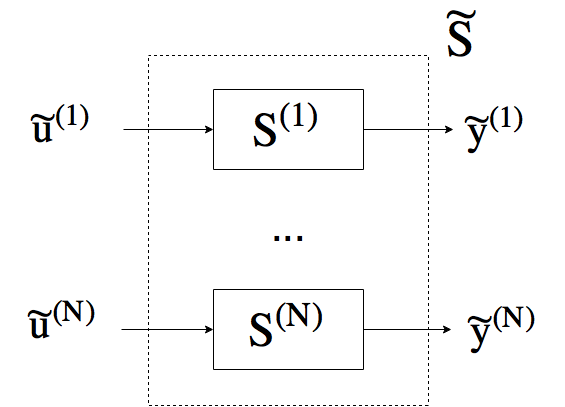
\includegraphics[width=.7\textwidth]{sistemi_interconnessi/sistema_ausiliario}
			\caption{sistema ausiliario}
			\label{fig:sistema_ausiliario}
		\end{figure}
		Prendiamo un sistema ausiliario come in figura \ref{fig:sistema_ausiliario} costituito da tutti i singoli $ S^{(i)} $ ognuno con un suo ingresso $ \tilde{\vec u^{(i)}} $ e una sua uscita $ \tilde{\vec y^{(i)}} = \vec{y}^{(i)} $. Il sistema $ \tilde S $ \'e completamente controllabile da $ \tilde{\vec u} $ e completamente osservabile da $ \tilde{\vec y} $.
		
		Il sistema interconnesso $ S $ con aggiunta di ingressi "ausiliari" $ \tilde{\vec u^{(i)}} $ e uscite "ausiliarie" $ \tilde{\vec y^{(i)}} $ corrisponde, se considero come ingressi $ \tilde{\vec u} $ e come uscite $ \tilde{\vec y} $, a una retroazione algebrica sull'uscita di $ \tilde S $. Sappiamo che la retroazione algebrica sull'uscita non modifica le propriet\'a di controllabilit\'a e osservabilit\'a, quindi il sistema cos\'i costituito \'e completamente controllabile da $ \tilde{\vec u} $ e osservabile da $ \tilde{\vec y} $.
		
		La controllabilit\'a \'e relativa agli ingressi e non dipende dalle particolari uscite. Se scelgo come ingressi quelli "veri" $ \vec u $ e come uscite quelle ausiliare $ \vec y $, allora da $ T_{\tilde y u}(s) $ ottengo le propriet\'a sulla controllabilit\'a. Analogamente se considero $ T_{y \tilde u}(s) $ ottengo propriet\'a sull'osservabilit\'a. Se scelgo $ T_{yu}(s) $ ottengo propriet\'a su controllabilit\'a e osservabilit\'a.
		\[
			\begin{array}{llll}
				T_{yu}(s) \quad\Rightarrow & \varphi_{CO}(s) & m_{CO}(s) & \Rightarrow\quad \text{stabilit\'a BIBO}
				\\ 
				T_{\tilde y u}(s) \quad\Rightarrow & \varphi_C(s) & m_C(s) & \Rightarrow\quad \text{Controllabilit\'a, stabilit\'a di } x_f
				\\ 
				T_{y \tilde u}(s) \quad\Rightarrow & \varphi_O(s) & m_O(s) & \Rightarrow\quad \text{Osservabilit\'a, stabilit\'a di } y_l
				\\ 
				T_{\tilde y \tilde u}(s) \quad\Rightarrow & \varphi(s) & m(s) & \Rightarrow\quad \text{Stabilit\'a interna}
			\end{array}
		\]
		
		\paragraph{Esempio}
			Prendiamo un sistema di ordine 2
			\[
			T(s) = \dfrac{1}{s-1} \quad\Rightarrow\quad \varphi_{CO}(s) \equiv m_{CO}(s) = s-1
			\]
			\begin{figure}[h!]
				\centering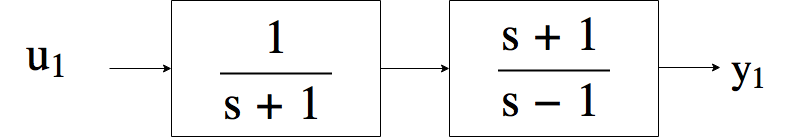
\includegraphics[width=.7\textwidth]{sistemi_interconnessi/esempio_sistema_ausiliario1}
			\end{figure}
			
			Costruiamo il sistema ausiliario:
			\begin{figure}[h!]
				\centering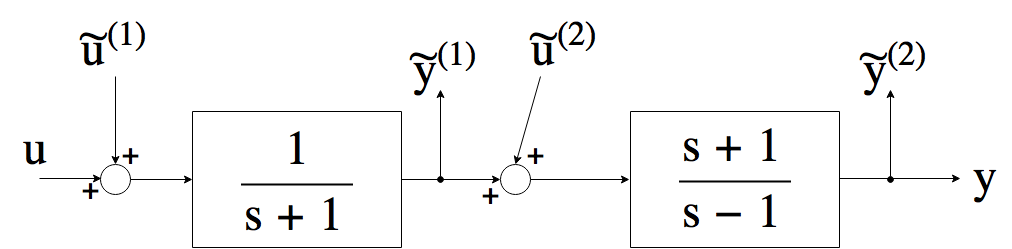
\includegraphics[width=.7\textwidth]{sistemi_interconnessi/esempio_sistema_ausiliario2}
			\end{figure}
			\begin{itemize}
				\item 
					Verifichiamo la controllabilit\'a:
					\[
						T_{\tilde yu}(s) =
						\begin{bmatrix}
							T_{\tilde y^{(1)}}(s)\\
							T_{\tilde y^{(2)}}(s)
						\end{bmatrix} =
						\begin{bmatrix}
							\dfrac{1}{s+1}\\
							\dfrac{1}{s-1}
						\end{bmatrix}
						\quad\Rightarrow\quad
						\varphi_C(s) \equiv m_C(s) = (s+1)(s-1)
					\]
					\'e completamente controllabile.
				\item 
					Verifichiamo l'osservabilit\'a:
					\[
						T_{y \tilde u}(s) = 
						\begin{bmatrix}
							T_{y \tilde u^{(1)}} & T_{y \tilde u^{(2)}}
						\end{bmatrix} =
						\begin{bmatrix}
							\dfrac{1}{s-1} & \dfrac{s+1}{s-1}
						\end{bmatrix}
						\quad\Rightarrow\quad
						\varphi_O(s) \equiv m_O(s) = (s-1)
					\]
				\item 
					Verifichiamo la contemporanea controllabilit\'a e osservabilit\'a:
					\[
						T_{\tilde y \tilde u} =
						\begin{bmatrix}
							\dfrac{1}{s+1} & 0\\
							\dfrac{1}{s-1} & \dfrac{s+1}{s-1}
						\end{bmatrix}
						\quad\Rightarrow\quad
						\varphi(s) \equiv m(s) = (s+1)(s-1)
					\]
			\end{itemize}
		
	\subsection{Cancellazione}
		\begin{itemize}
			\item 
				cancellazione polo-zero nella serie:
				\begin{figure}[h!]
					\centering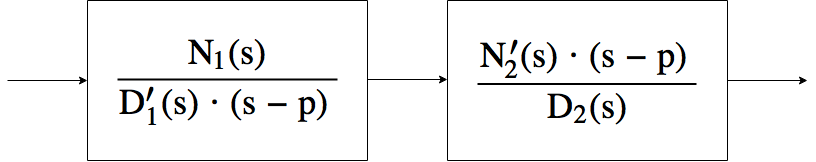
\includegraphics[width=.5\textwidth]{sistemi_interconnessi/cancellazione_polo_zero}
				\end{figure}
			
				\[
					\varphi(s) = D^{'}(s) \cdot (s-p) \cdot D_2(s) \qquad T(s) = \dfrac{N_1(s) N_2^{'}(s)}{D_1^{'}(s) D_2(s)}
				\]
				L'autovalore $ s=p $ non \'e contemporaneamente controllabile e osservabile. Verifichiamo se \'e controllabile:
				\[
					T_{\tilde y u}(s) =
					\begin{bmatrix}
						\dfrac{N_1(s)}{D_1^{'}(s) \cdot (s-p)}\\[.5cm]
						\dfrac{N_1(s)N_2(s)}{D_1^{'}(s) D_2(s)}
					\end{bmatrix}
					\qquad
					\varphi_C(s) = D_1^{'}(s) \cdot D_2(s) \cdot (s-p)
				\]
				Quindi $ p $ \'e controllabile ma per quanto detto prima non \'e osservabile.
			\item 
				cancellazione zero-polo nella serie:
				\begin{figure}[h!]
					\centering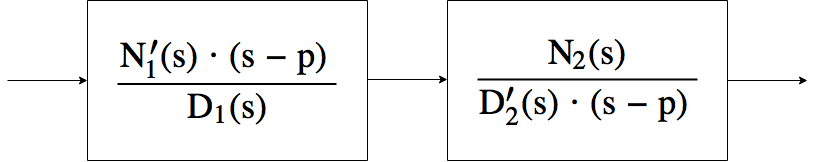
\includegraphics[width=.5\textwidth]{sistemi_interconnessi/cancellazione_zero_polo}
				\end{figure}
			
				\[
					T(s) =
					\dfrac{N_1^{'}(s) N_2(s)}{D_2(s) D_1^{'}(s)}
				\]
				$ s=p $ \'e osservabile ma non controllabile. Verifichiamolo:
				\[
					T_{y \tilde u}(s) =
					\begin{bmatrix}
						\dfrac{N_1^{'}(s) N_2(s)}{D_1(s) D_2^{'}(s)} & \dfrac{N_2(s)}{D_2^{'}(s) \cdot (s-p)}
					\end{bmatrix}
					\qquad
					\varphi_O(s) = D_2^{'}(s) \cdot D_1(s) \cdot (s-p)
				\]
			\item 
				cancellazione nel parallelo:
				\begin{figure}[h!]
					\centering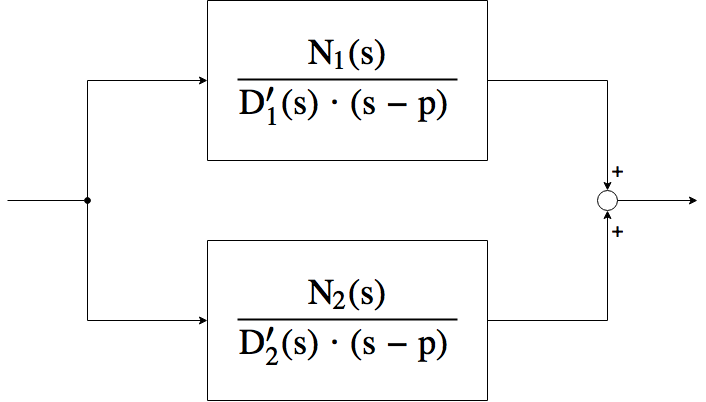
\includegraphics[width=.5\textwidth]{sistemi_interconnessi/cancellazione_parallelo}
				\end{figure}
			
				ipotizziamo che $ (s-p) $ sia fattore comune (non \'e presente in $ D_1^{'}(s) $ e $ D_2^{'}(s) $)
				\[
					T_{yu}(s) = T_1(s) + T_2(s) = 
					\dfrac{N_1(s)D_2^{'}(s) + N_2(s)D_1^{'}(s)}{D_1^{'}(s) D_2^{'}(s) (s-p)}
				\]
				\[
					\varphi_{CO}(s) = D_1^{'}(s) D_2^{'}(s) (s-p) \qquad \varphi(s) = D_1^{'}(s) D_2^{'}(s) (s-p)^2
				\]
				\begin{itemize}
					\item 
						controllabilit\'a:
						\[
							T_{\tilde y u}(s) =
							\begin{bmatrix}
								\dfrac{N_1(s)}{D_1^{'}(s) (s-p)}\\
								\dfrac{N_2(s)}{D_2^{'}(s) (s-p)}
							\end{bmatrix}
							\qquad
							\varphi_C(s) = D_1^{'}(s) D_2^{'}(s) (s-p)
						\]
						cio\'e perdo controllabilit\'a.
					\item 
						osservabilit\'a.
						\[
							T_{y \tilde u}(s) = 
							\begin{bmatrix}
								\dfrac{N_1(s)}{D_1^{'}(s) (s-p)} &
								\dfrac{N_2(s)}{D_2^{'}(s) (s-p)}
							\end{bmatrix}
						\]
						perdo osservabilit\'a.
				\end{itemize}
			Se ho due termini comuni al denominatore di due funzioni di trasferimento in parallelo perdo sia la controllabilit\'a che l'osservabilit\'a.
		\end{itemize}
	
	\section{Retroazione}
		L'unica situazione in cui il sistema non \'e completamente controllabile e osservabile gli zeri in catena diretta coincidono con i poli in catena inversa.
		\begin{figure}[h!]
			\centering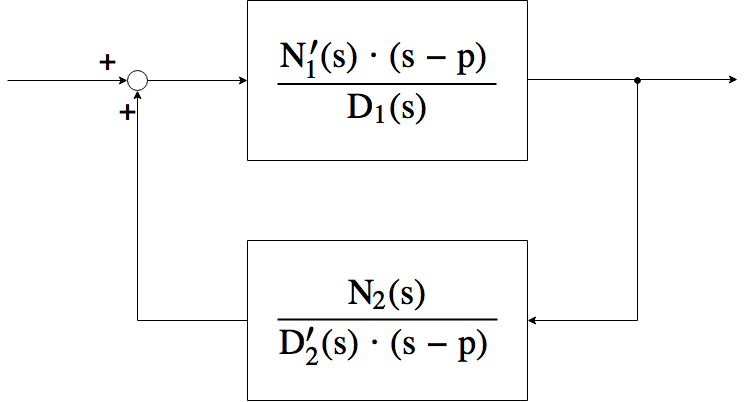
\includegraphics[width=.5\textwidth]{sistemi_interconnessi/retroazione}
		\end{figure}
	
		\[
			T(s) = \dfrac{\dfrac{N_1^{'}(s) (s-p)}{D_1(s)}}{1-\dfrac{N_1^{'}(s) (s-p)}{D_1(s)}\dfrac{N_2(s)}{D_2^{'}(s)(s-p)}} = \dfrac{N_1^{'}(s) (s-p) D_2^{'}(s)}{D_1(s)D_2^{'}(s) - N_1^{'}(s)N_2(s)}
		\]
		\begin{itemize}
			\item 
				Analisi osservabilit\'a (trascuro le $ u $)
				\begin{figure}[h!]
					\centering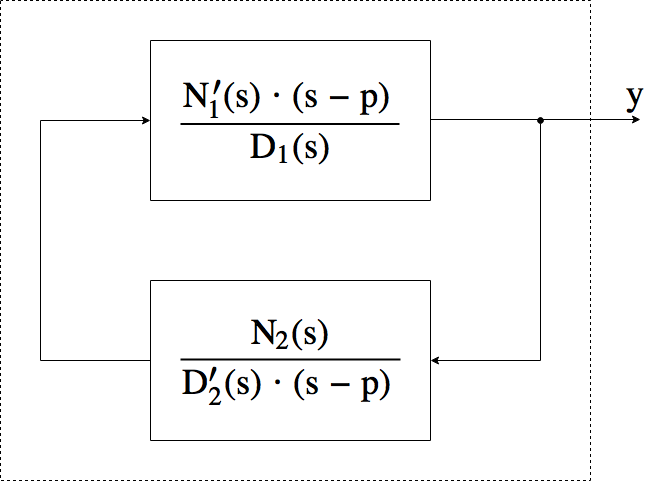
\includegraphics[width=.5\textwidth]{sistemi_interconnessi/retroazione_analisi_osservabilita}
					\caption{analisi osservabilit\'a}
					\label{fig:retroazione_analisi_osservabilita}
				\end{figure}
			
				Questo sottosistema \ref{fig:retroazione_analisi_osservabilita} ha 2 blocchi in serie con perdit\'a di osservabilit\'a (cancellazione polo-zero) $ \quad\Rightarrow\quad $ il sistema complessivo non \'e osservabile.
			\item 
				Analisi controllabilit\'a (trascuro le $ y $)
				\begin{figure}[h!]
					\centering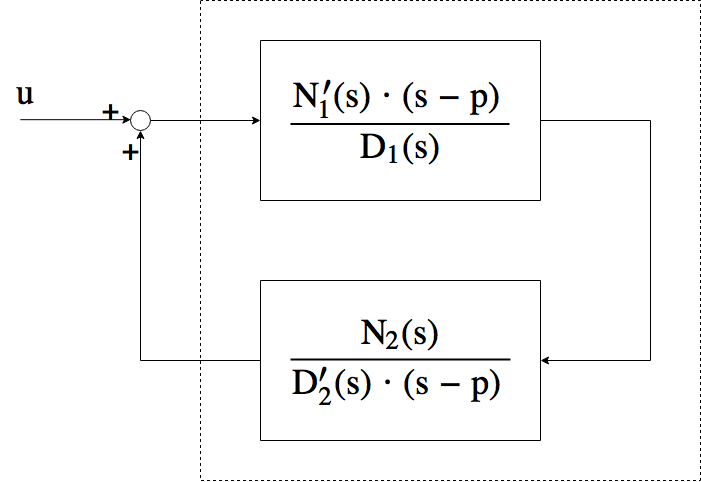
\includegraphics[width=.5\textwidth]{sistemi_interconnessi/retroazione_analisi_controllabilita}
					\caption{analisi controllabilit\'a}
					\label{fig:retroazione_analisi_controllabilita}
				\end{figure}
				
				Il sottosistema \ref{fig:retroazione_analisi_controllabilita} presenta una cancellazione zero-polo quindi il sistema complessivo non \'e controllabile.
		\end{itemize}
	
	\section{Effetto cancellazione}
		\begin{figure}[h!]
			\centering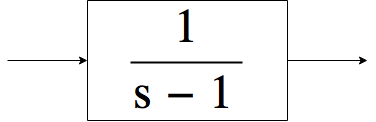
\includegraphics[width=.4\textwidth]{sistemi_interconnessi/effetto_cancellazione1}
			\label{fig:effetto_cancellazione1}
		\end{figure}
	
		Cerchiamo di cancellare un polo instabile dal sistema in figura \ref{fig:effetto_cancellazione1} aggiungendo un altro sistema in serie.
		\begin{figure}[h!]
			\centering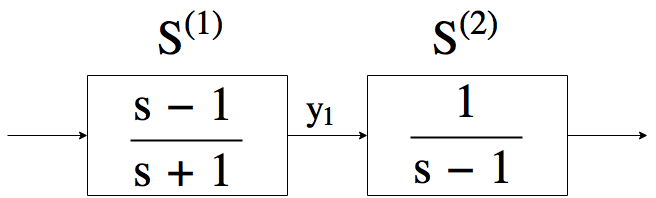
\includegraphics[width=.7\textwidth]{sistemi_interconnessi/effetto_cancellazione2}
			\label{fig:effetto_cancellazione2}
		\end{figure}
	
		Questo metodo non pu\'o essere utilizzato per eliminare l'instabilit\'a, perch\'e il sistema che abbiamo aggiunto dovrebbe avere uno zero precisamente in $ +1 $ (nella pratica sar\'a un\'approssimazione). Il residuo del polo $ +1 $ che non viene "cancellata", seppur piccolissimo, diverger\'a con una relazione esponenziale $ e^t $.
		
		Inoltre aggiungendo il sistema all'ingresso di $ T(s)=\dfrac{1}{s-1} $, perdiamo la controllabilit\'a del polo $ +1 $. Quindi se $ u = 0 $, ma la condizione iniziale del sistema $ S^{(1)} $ non \'e nulla $ x^{(1)} \neq 0 $, il secondo sistema $ S^{(2)} $ diverger\'a.
		
		Potremmo allora decidere di postporre il sistema $ S^{(2)} $:
		\begin{figure}[h!]
			\centering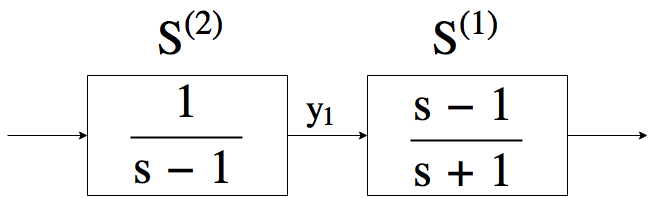
\includegraphics[width=.7\textwidth]{sistemi_interconnessi/effetto_cancellazione3}
			\label{fig:effetto_cancellazione3}
		\end{figure}
	
		In questo nuovo sistema la parte instabile \'e non osservabile, mentre quella stabile \'e osservabile. Se $ u \neq 0 $ oppure $ u = 0 $ ma $ x_1 \neq 0 $, la quantit\'a interna $ y_1 $ diverge: dall'uscita complessiva del sistema vedo sempre un'uscita limitata ma la quantit\'a interna diverge.
		
		Concludiamo che cancellare algebricamente un autovalore non significa eliminarlo, ma nasconderlo dalla funzione di trasferimento.
		
	\subsection{Dove "finiscono" gli autovalori "cancellati"}
		\begin{figure}[h!]
			\centering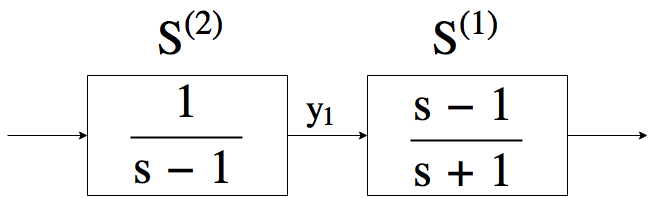
\includegraphics[width=.7\textwidth]{sistemi_interconnessi/effetto_cancellazione3}
		\end{figure}
		\[
			T(s) = \dfrac{1}{s+1}
			\qquad\Rightarrow\qquad
			\varphi_{CO}(s)=s+1
		\]
		in $ \varphi_{CO}(s) $ non compare pi\'u l'autovalore $ +1 $, che \'e stato cancellato. Se invece consideriamo il polinomio caratteristico:
		\[
			\varphi(s)=(s+1)(s-1)
		\]
		$ s_1 = -1 $ \'e controllabile e osservabile, mentre $ s_2 = +1 $ \'e solo controllabile.
		
		Effettuiamo una retroazione algebrica sull'uscita:
		\begin{figure}[h!]
			\centering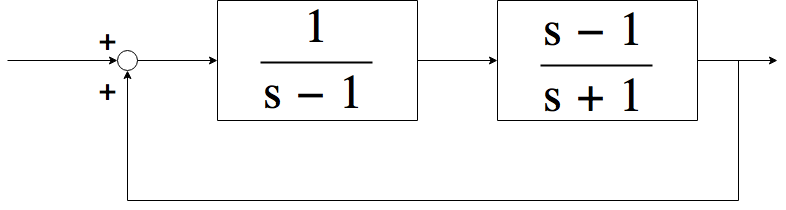
\includegraphics[width=.7\textwidth]{sistemi_interconnessi/effetto_cancellazione4}
		\end{figure}
		
		\[
			T(s)=\dfrac{\dfrac{1}{s+1}}{1-\dfrac{1}{s+1}} = \dfrac{1}{s} \quad\Rightarrow\quad \varphi_C(s)=s \varphi(s)=s(s-1)
		\]
		
		Abbiamo gi\'a visto che la retroazione algebrica sull'uscita modifica solo gli autovalori controllabili e osservabili: infatti $ s_2 $ non viene modificato, mentre $ s_2 $ passa da $ -1 $ a $ 0 $.
		
		\begin{center}
			\fbox{
				\begin{minipage}{.8\textwidth}
					Gli autovalori "cancellati" non si spostano, rimangono parte del polinomio caratteristico.
				\end{minipage}
			}
		\end{center}
		
\end{document}